% ╔══════════════════════════════════════════════════════════════════╗
% ║  Pollination Networks — IIT Bhilai                              ║
% ║  16:9 Academic Poster  ·  300 DPI  ·  Overleaf-ready           ║
% ║  Paper size: 48in × 27in  (scales cleanly to any 16:9 output)  ║
% ╚══════════════════════════════════════════════════════════════════╝
\documentclass[final]{beamer}

% ── Page geometry: 48×27 inches, 16:9, 300 DPI ───────────────────
\usepackage[
  paperwidth  = 48in,
  paperheight = 27in,
  margin      = 0pt
]{geometry}

% ── Core packages ─────────────────────────────────────────────────
\usepackage{fontenc}
\usepackage[utf8]{inputenc}
\usepackage{lmodern}
\usepackage{microtype}
\usepackage{xcolor}
\usepackage{graphicx}
\usepackage{tikz}
\usetikzlibrary{shapes.geometric, arrows.meta, positioning, calc,
                decorations.pathreplacing, backgrounds, patterns,
                fit, matrix, shapes.misc}
\usepackage{pgfplots}
\pgfplotsset{compat=1.18}
\usepackage{booktabs}
\usepackage{array}
\usepackage{tabularx}
\usepackage{multirow}
\usepackage{colortbl}
\usepackage{mdframed}
\usepackage{enumitem}
\usepackage{multicol}
\usepackage{ragged2e}
\usepackage{calc}
\usepackage{varwidth}
\usepackage{tcolorbox}
\tcbuselibrary{skins, breakable, hooks}
\usepackage{amsmath, amssymb}

% ── Fonts ─────────────────────────────────────────────────────────
\usepackage{ebgaramond}   % Cormorant Garamond substitute (serif)
\usepackage{cabin}        % Jost substitute (sans-serif)
\usepackage{inconsolata}  % JetBrains Mono substitute (mono)
\renewcommand{\familydefault}{\sfdefault}  % default to sans

% ── Colour palette ────────────────────────────────────────────────
\definecolor{ink}    {HTML}{0d1a0f}
\definecolor{forest} {HTML}{122a18}
\definecolor{panel}  {HTML}{f7f4ee}
\definecolor{panel2} {HTML}{eef5f0}
\definecolor{panel3} {HTML}{0f2217}
\definecolor{gold}   {HTML}{c8952a}
\definecolor{gold2}  {HTML}{f0c050}
\definecolor{lime}   {HTML}{7ec850}
\definecolor{teal}   {HTML}{2ec4a0}
\definecolor{coral}  {HTML}{e8624a}
\definecolor{sky}    {HTML}{4fa8d8}
\definecolor{cream}  {HTML}{faf6ef}
\definecolor{ivory}  {HTML}{fffdf7}
\definecolor{bodytext}{HTML}{2a3e2e}
\definecolor{muted}  {HTML}{5a7060}
\definecolor{darkgrn}{HTML}{1a3020}
\definecolor{headgold}{HTML}{b5820f}
\definecolor{headteal}{HTML}{1a7a65}
\definecolor{headcoral}{HTML}{b84030}
\definecolor{headsky}{HTML}{2a7aa8}
\definecolor{headlime}{HTML}{4e9828}
\definecolor{headplum}{HTML}{6a3a8a}
\definecolor{headslate}{HTML}{2e4a5a}
\definecolor{headamber}{HTML}{a06010}
\definecolor{plumlight}{HTML}{c084fc}
\definecolor{skylight}{HTML}{4fa8d8}
\definecolor{amberlight}{HTML}{f0a030}
\definecolor{amberbg} {HTML}{fef8e8}
\definecolor{tealbg}  {HTML}{e8f8f4}
\definecolor{coralbg} {HTML}{fdf0ee}
\definecolor{skybg}   {HTML}{e8f4fc}
\definecolor{limebg}  {HTML}{f0f8ec}
\definecolor{darkgreen}{HTML}{4e9828}

% ── Suppress Beamer decorations ───────────────────────────────────
\setbeamertemplate{navigation symbols}{}
\setbeamertemplate{headline}{}
\setbeamertemplate{footline}{}
\setbeamercolor{background canvas}{bg=white}
\setbeamersize{text margin left=0pt, text margin right=0pt}

% ── Convenience dimensions ────────────────────────────────────────
\newlength{\PW}\setlength{\PW}{48in}
\newlength{\PH}\setlength{\PH}{27in}
% Column widths (3 cols: 1.05 : 1.00 : 0.95 of equal share)
\newlength{\ColSep}\setlength{\ColSep}{0.18in}
\newlength{\ColW}  % set in document

% ── tcolorbox card style ──────────────────────────────────────────
\tcbset{
  postercard/.style={
    enhanced, sharp corners=all,
    boxrule=0pt, frame hidden,
    colback=panel,
    drop shadow={opacity=0.22, shadow xshift=2pt, shadow yshift=-2pt},
    before upper={\setlength{\parskip}{4pt}},
    left=9pt, right=9pt, top=0pt, bottom=8pt,
    fontupper=\small\color{bodytext},
  },
  cardhead/.style={
    enhanced, sharp corners=all, frame hidden,
    left=9pt, right=9pt, top=4pt, bottom=4pt,
    fontupper=\color{ivory}\ebgaramondFont\bfseries\fontsize{13}{15}\selectfont,
  },
  calloutgold/.style={
    enhanced, sharp corners=all, frame hidden,
    colback=amberbg, borderline west={3pt}{0pt}{gold},
    left=7pt, right=7pt, top=5pt, bottom=5pt,
    fontupper=\fontsize{9}{12}\selectfont\color{darkgrn},
  },
  calloutteal/.style={
    enhanced, sharp corners=all, frame hidden,
    colback=tealbg, borderline west={3pt}{0pt}{teal},
    left=7pt, right=7pt, top=5pt, bottom=5pt,
    fontupper=\fontsize{9}{12}\selectfont\color{darkgrn},
  },
  calloutcoral/.style={
    enhanced, sharp corners=all, frame hidden,
    colback=coralbg, borderline west={3pt}{0pt}{coral},
    left=7pt, right=7pt, top=5pt, bottom=5pt,
    fontupper=\fontsize{9}{12}\selectfont\color{darkgrn},
  },
  calloutsky/.style={
    enhanced, sharp corners=all, frame hidden,
    colback=skybg, borderline west={3pt}{0pt}{sky},
    left=7pt, right=7pt, top=5pt, bottom=5pt,
    fontupper=\fontsize{9}{12}\selectfont\color{darkgrn},
  },
}

% ── Bullet list style ─────────────────────────────────────────────
\newlist{pbullet}{itemize}{1}
\setlist[pbullet]{
  label={\textcolor{gold}{\scriptsize$\blacktriangleright$}},
  leftmargin=14pt, itemsep=1pt, topsep=2pt,
  font=\fontsize{10}{13}\selectfont\color{bodytext}
}

% ── Font shorthand ────────────────────────────────────────────────
\newcommand{\ebgaramondFont}{\fontfamily{EBGaramond-OsF}\selectfont}
\newcommand{\monoFont}{\ttfamily}
\newcommand{\histat}[1]{{\monoFont\bfseries\color{teal}#1}}
\newcommand{\lostat}[1]{{\monoFont\bfseries\color{coral}#1}}
\newcommand{\gcstat}[1]{{\monoFont\bfseries\color{darkgreen}#1}}
\newcommand{\ocstat}[1]{{\monoFont\bfseries\color{headamber}#1}}

% ── Card construction helpers ─────────────────────────────────────
% #1=head bg colour, #2=number bg colour, #3=number text, #4=title
\newcommand{\cardhead}[4]{%
  \begin{tcolorbox}[cardhead, colback=#1]
    \begin{tikzpicture}[baseline=(n.base)]
      \node[circle, fill=#2, inner sep=0pt,
            minimum size=16pt, font=\monoFont\fontsize{8}{8}\selectfont\color{forest}]
        (n) {#3};
    \end{tikzpicture}\hspace{6pt}#4
  \end{tcolorbox}%
}

% ─────────────────────────────────────────────────────────────────
\begin{document}
\begin{frame}[t]{}

% ════════════════════════════════════════════════════════
%   FULL-POSTER TIKZ CANVAS
% ════════════════════════════════════════════════════════
\begin{tikzpicture}[remember picture, overlay,
    every node/.style={inner sep=0pt, outer sep=0pt}]

  % Poster origin at top-left
  \coordinate (TL) at (current page.north west);
  \coordinate (TR) at (current page.north east);
  \coordinate (BL) at (current page.south west);
  \coordinate (BR) at (current page.south east);

  % ── Background: faint network science tile ──────────────────
  \begin{scope}[opacity=0.10]
    \foreach \dx in {0, 3.2, 6.4, 9.6, 12.8, 16, 19.2, 22.4, 25.6, 28.8,
                     32, 35.2, 38.4, 41.6, 44.8} {
      \foreach \dy in {0, 2.2, 4.4, 6.6, 8.8, 11, 13.2, 15.4, 17.6, 19.8,
                       22, 24.2, 26.4} {
        \begin{scope}[xshift=\dx in, yshift=-\dy in]
          \draw[sky, line width=0.7pt]
            (0.24,  -0.34) -- (0.92, -0.66) -- (1.58, -0.42)
            (1.58, -0.42)  -- (2.22, -0.86)
            (0.92, -0.66)  -- (1.22, -1.36) -- (2.10, -1.50)
            (2.22, -0.86)  -- (2.10, -1.50) -- (2.86, -1.18)
            (1.58, -0.42)  -- (1.22, -1.36);
          \foreach \cx/\cy/\cr in {
            0.24/-0.34/2.5pt, 0.92/-0.66/3.5pt, 1.58/-0.42/2.5pt,
            2.22/-0.86/3.5pt, 1.22/-1.36/4pt,   2.10/-1.50/3.5pt, 2.86/-1.18/2.5pt}{
            \fill[lime!80] (\cx,\cy) circle (\cr);
          }
        \end{scope}
      }
    }
  \end{scope}

  % ── Subtle radial glows ──────────────────────────────────────
  \fill[lime, opacity=0.04]  (5.76in, -21.06in) ellipse (13.44in and 8.64in);
  \fill[sky,  opacity=0.04]  (42.24in,-5.94in)  ellipse (15.36in and 9.60in);

  % ════════════════════════════════════════════════════════
  %   HEADER  (top 3.5 in)
  % ════════════════════════════════════════════════════════
  % Header background gradient
  \fill[white]          (TL) rectangle ++(48in, -3.5in);
  \fill[panel2, opacity=0.55] ($(TL)+(0,-1.75in)$) rectangle ++(48in,-1.75in);
  % Gold bottom border
  \fill[gold] ($(BL)+(0,23.5in)$) rectangle ++(48in, 3pt);

  % ── Decorative network (top-right of header) ──────────────
  \begin{scope}[xshift=31.5in, yshift=-0.3in, opacity=0.12, scale=2.2]
    \draw[lime, line width=1pt]
      (0.60,-0.20) -- (1.20,-0.60) -- (2.00,-0.30) -- (2.80,-0.80) -- (3.60,-0.40)
      (0.60,-0.20) -- (1.60,-1.00) -- (2.40,-1.30) -- (4.00,-1.10)
      (2.00,-0.30) -- (1.60,-1.00) (2.80,-0.80) -- (2.40,-1.30)
      (3.60,-0.40) -- (4.00,-1.10)
      (1.20,-0.60) -- (1.60,-1.00) (0.60,-1.20) -- (1.60,-1.00)
      (0.60,-1.20) -- (1.20,-0.60);
    \foreach \cx/\cy/\cr in {
      0.60/-0.20/4pt, 1.20/-0.60/6pt, 2.00/-0.30/4pt,
      2.80/-0.80/7pt, 3.60/-0.40/3pt, 0.60/-1.20/4pt,
      1.60/-1.00/8pt, 2.40/-1.30/5pt, 4.00/-1.10/3pt}{
      \fill[lime] (\cx in,\cy in) circle (\cr);
    }
  \end{scope}

  % ── Logo panel (left strip of header) ─────────────────────
  \fill[gold!15] (TL) rectangle ++(3.84in,-3.5in);
  \draw[gold!50, line width=0.8pt] ($(TL)+(3.84in,0)$) -- ++(0,-3.5in);

  % IIT Bhilai logo
  \node[anchor=center] at ($(TL)+(1.92in,-1.75in)$) {%
    \includegraphics[width=3.2in, height=3.2in, keepaspectratio]{iit_bhilai_logo.png}%
  };

  % ── Header main text ──────────────────────────────────────
  % Tag pill
  \node[anchor=west,
        fill=gold!20, draw=gold!60, rounded corners=10pt,
        inner xsep=8pt, inner ysep=2pt,
        font=\sffamily\bfseries\fontsize{9}{9}\selectfont\color{gold2},
        text depth=1.5pt]
    at ($(TL)+(4.20in,-0.45in)$)
    {{\fontsize{6}{6}\selectfont\color{gold}$\blacklozenge$}\quad
     NETWORK SCIENCE\enspace·\enspace APRIL 2026};

  % Title
  \node[anchor=north west,
        text width=27in,
        font=\ebgaramondFont\bfseries\fontsize{52}{58}\selectfont\color{forest},
        align=left]
    at ($(TL)+(4.20in,-0.80in)$)
    {Stability and {\color{gold2}Collapse} of\\Pollination Networks};

  % Subtitle
  \node[anchor=north west,
        text width=26in,
        font=\sffamily\fontsize{14}{18}\selectfont\color{forest!70},
        align=left]
    at ($(TL)+(4.22in,-2.18in)$)
    {A Network Science Perspective \enspace·\enspace
     Indian Institute of Technology Bhilai};

  % Authors
  \foreach \name/\xpos in {
    {Agastya Nath}/0,
    {Aman Pratap Singh}/2.5,
    {Dhananjoy Doley}/5.4,
    {Paritosh Lahre}/8.0,
    {Rahul Dev Reddy}/10.2}
  {
    \node[anchor=west,
          fill=forest!7, draw=forest!18, rounded corners=8pt,
          inner xsep=8pt, inner ysep=2.5pt,
          font=\sffamily\fontsize{11}{11}\selectfont\color{forest!85}]
      at ($(TL)+(4.22in+\xpos in,-2.75in)$)
      {\name};
  }

  % ── Stats panel (right of header) ────────────────────────
  \fill[gold!12] ($(TR)+(0,0)$) rectangle ++(-8.64in,-3.5in);
  \draw[gold!40, line width=0.8pt]
    ($(TR)+(-8.64in,0)$) -- ++(0,-3.5in);

  % Stats
  \foreach \val/\lbl/\yoff in {
    {172}/{Networks}/{0.5},
    {6}/{Continents}/{1.25},
    {0.960}/{GNN AUC}/{2.00},
    {11.5K}/{Species}/{2.75}}{
    \node[anchor=center,
          font=\monoFont\bfseries\fontsize{30}{30}\selectfont\color{gold2}]
      at ($(TR)+(-4.32in,-\yoff in)$) {\val};
    \node[anchor=center,
          font=\sffamily\fontsize{10}{10}\selectfont\color{forest!65}]
      at ($(TR)+(-4.32in,-\yoff in -0.28in)$)
      {\MakeUppercase{\lbl}};
  }
  % Dividers between stats
  \foreach \yoff in {0.875, 1.625, 2.375}{
    \draw[gold!40, line width=0.6pt]
      ($(TR)+(-7.8in,-\yoff in)$) -- ($(TR)+(-0.86in,-\yoff in)$);
  }

  % ════════════════════════════════════════════════════════
  %   ABSTRACT STRIP  (3.5in – 4.7in from top)
  % ════════════════════════════════════════════════════════
  \fill[gold] ($(TL)+(0,-3.5in)$) rectangle ++(48in,-1.20in);

  \node[anchor=west,
        font=\ebgaramondFont\bfseries\fontsize{13}{13}\selectfont\color{black!50},
        text depth=0pt]
    at ($(TL)+(1.0in,-4.10in)$) {ABSTRACT};

  \node[anchor=west,
        text width=44in,
        font=\sffamily\fontsize{12.5}{17}\selectfont\color{black!85},
        align=left]
    at ($(TL)+(3.8in,-4.10in)$)
    {Pollination networks sustain \textbf{\textasciitilde88\% of flowering plants} and
     \textbf{75\% of global food crops}. We analyse \textbf{172 real-world bipartite
     networks} across 6 continents using cascading co-extinction simulation,
     climate stress modelling, adaptive rewiring, early warning signal detection,
     Random Forest extinction risk prediction, \textbf{GraphSAGE-based role discovery},
     and species transplantation to characterise structural vulnerability and
     collapse dynamics at continent scale.};

  % ════════════════════════════════════════════════════════
  %   COLUMN SEPARATORS  (4.7in – 22.3in from top)
  % ════════════════════════════════════════════════════════
  % Column boundaries: col1=0–16.8in, col2=16.8–32.64in, col3=32.64–48in
  \draw[gold!35, line width=0.7pt]
    ($(TL)+(16.32in,-4.7in)$) -- ++(0,-17.6in);
  \draw[gold!35, line width=0.7pt]
    ($(TL)+(32.16in,-4.7in)$) -- ++(0,-17.6in);

\end{tikzpicture}

% ════════════════════════════════════════════════════════
%   BODY — three columns via minipage
% ════════════════════════════════════════════════════════
\vspace*{4.73in}  % push below header + abstract strip

{%
\setlength{\ColW}{15.84in}%
\setlength{\parindent}{0pt}%
\fontsize{10.5}{14}\selectfont%
%
% ──────────────────── three columns ───────────────────
\begin{minipage}[t]{\ColW}
  \hspace*{0.55in}% left inset

  % ╔═══════════════════════════════╗
  % ║  CARD 1 · Dataset & Model     ║
  % ╚═══════════════════════════════╝
  \begin{tcolorbox}[
    enhanced, sharp corners, frame hidden,
    colback=panel, left=8pt, right=8pt, top=0pt, bottom=8pt,
    width=15.0in,
    drop shadow={opacity=0.20},
    before={\vspace{2pt}}, after={\vspace{8pt}}]
    % Head
    \begin{tcolorbox}[
      enhanced, sharp corners, frame hidden,
      colback=headgold, left=8pt, right=8pt, top=4pt, bottom=4pt,
      width=\linewidth]
      
\begin{tikzpicture}[baseline=(n.base)]
        \node[circle, fill=gold2, inner sep=0pt,
              minimum size=14pt,
              font=\monoFont\fontsize{8}{8}\selectfont\bfseries\color{forest}]
          (n) {1};
      \end{tikzpicture}\enspace
      {\ebgaramondFont\bfseries\fontsize{14}{16}\selectfont\color{ivory}%
       Dataset \& Network Model}
    \end{tcolorbox}

    \vspace{5pt}
    {\color{bodytext} Bipartite graph \textbf{G = (U $\cup$ V, E)}: pollinators (U),
     plants (V). \textbf{172 city-level datasets} from Web of Life were grouped into
     6 continental meta-networks for macro-scale comparison, while all 172 were
     retained for network-level GNN analysis.}

    \vspace{6pt}
    % Pipeline diagram
    \begin{center}
    
\begin{tikzpicture}[
      box/.style={
        draw=gold, fill=darkgrn, rounded corners=4pt,
        text=gold2, font=\sffamily\fontsize{8}{9}\selectfont,
        inner xsep=5pt, inner ysep=4pt, align=center,
        minimum width=1.6in, minimum height=0.45in},
      arr/.style={-Stealth, gold, line width=1pt},
      node distance=0.2in]
      \node[box] (db)   {Web of Life\\\small Database};
      \node[box, right=0.15in of db] (bg) {Bipartite\\\small Graph G};
      \node[box, right=0.15in of bg] (me) {Metrics\\\small Compute};
      \node[box, right=0.15in of me] (cn) {Continental\\\small Grouping};
      \node[box, right=0.15in of cn] (an) {Analysis\\\small Pipeline};
      \draw[arr] (db) -- (bg);
      \draw[arr] (bg) -- (me);
      \draw[arr] (me) -- (cn);
      \draw[arr] (cn) -- (an);
    \end{tikzpicture}
    \end{center}

    \vspace{4pt}
    % Bipartite diagram
    \begin{center}
    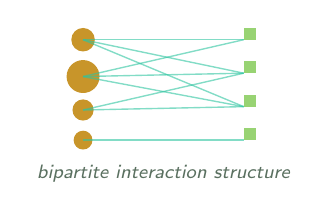
\begin{tikzpicture}[scale=0.85]
      \foreach \y/\r in {0/5pt, -0.55/7pt, -1.05/4.5pt, -1.5/4pt}
        \fill[gold] (-1.2,\y) circle (\r);
      \foreach \y in {0, -0.5, -1.0, -1.5}
        \fill[lime!80] (1.2,\y) rectangle ++(0.18, 0.18);
      \foreach \py/\vy in {0/0, 0/-0.5, 0/-1.0, -0.55/0, -0.55/-0.5,
                           -0.55/-1.0, -1.05/-0.5, -1.05/-1.0, -1.5/-1.5}
        \draw[teal, opacity=0.6, line width=0.5pt] (-1.2,\py) -- (1.2,\vy);
      \node[font=\sffamily\fontsize{7}{7}\selectfont\itshape\color{muted}]
        at (0,-2.0) {bipartite interaction structure};
    \end{tikzpicture}
    \end{center}

    \vspace{2pt}
    \begin{pbullet}
      \item \textbf{Degree Centrality} — generalist identification
      \item \textbf{Betweenness Centrality} — bridge species
      \item \textbf{Eigenvector Centrality} — systemic influence
      \item \textbf{NODF Nestedness} — specialist–generalist hierarchy
      \item \textbf{Modularity Q} — community compartmentalisation
    \end{pbullet}
  \end{tcolorbox}

  % ╔════════════════════════════════════════╗
  % ║  CARD 2 · Continental Network Props    ║
  % ╚════════════════════════════════════════╝
  \begin{tcolorbox}[
    enhanced, sharp corners, frame hidden,
    colback=panel, left=8pt, right=8pt, top=0pt, bottom=8pt,
    width=15.0in,
    drop shadow={opacity=0.20},
    before={\vspace{2pt}}, after={\vspace{8pt}}]
    % Head
    \begin{tcolorbox}[enhanced, sharp corners, frame hidden,
      colback=headteal, left=8pt, right=8pt, top=4pt, bottom=4pt, width=\linewidth]
      
\begin{tikzpicture}[baseline=(n.base)]
        \node[circle, fill=teal, inner sep=0pt, minimum size=14pt,
              font=\monoFont\fontsize{8}{8}\selectfont\bfseries\color{forest}](n){2};
      \end{tikzpicture}\enspace
      {\ebgaramondFont\bfseries\fontsize{14}{16}\selectfont\color{ivory}%
       Continental Network Properties}
    \end{tcolorbox}

    \vspace{6pt}
    \renewcommand{\arraystretch}{1.18}
    \fontsize{10}{13}\selectfont
    \begin{tabularx}{\linewidth}{>{\bfseries}X r r r r r}
      \rowcolor{darkgrn}%
      \textcolor{gold2}{\small Continent} &
      \textcolor{gold2}{\small Plants} &
      \textcolor{gold2}{\small Pollin.} &
      \textcolor{gold2}{\small NODF} &
      \textcolor{gold2}{\small Q} &
      \textcolor{gold2}{\small Conn.} \\
      Africa      & 147  & 737  & \ocstat{18.2↑}& 0.453           & 0.15 \\
      \rowcolor{panel2}
      Asia        & 543  & \lostat{2947} & 4.3   & \histat{0.602}  & 0.12 \\
      Europe      & 417  & 1988 & 5.4           & \histat{0.627}  & 0.13 \\
      \rowcolor{panel2}
      N. America  & \lostat{909} & 1855 & \lostat{3.2↓} & \lostat{0.270↓} & \lostat{0.09} \\
      Oceania     & 127  & 299  & 9.4           & 0.488           & 0.16 \\
      \rowcolor{panel2}
      S. America  & \histat{1089} & 907 & 3.9   & \gcstat{0.773↑} & \lostat{0.08} \\
    \end{tabularx}

    \vspace{6pt}
    \begin{tcolorbox}[calloutgold]
      \textbf{South America} (Q=0.773) most modular; \textbf{North America}
      (Q=0.270) most integrated and most vulnerable to targeted attack.
    \end{tcolorbox}
  \end{tcolorbox}

  % ╔══════════════════════════════════════╗
  % ║  CARD 3 · GNN Functional Role Disc.  ║
  % ╚══════════════════════════════════════╝
  \begin{tcolorbox}[
    enhanced, sharp corners, frame hidden,
    colback=panel, left=8pt, right=8pt, top=0pt, bottom=8pt,
    width=15.0in,
    drop shadow={opacity=0.20},
    before={\vspace{2pt}}, after={\vspace{8pt}}]
    % Head
    \begin{tcolorbox}[enhanced, sharp corners, frame hidden,
      colback=headplum, left=8pt, right=8pt, top=4pt, bottom=4pt, width=\linewidth]
      
\begin{tikzpicture}[baseline=(n.base)]
        \node[circle, fill=plumlight, inner sep=0pt, minimum size=14pt,
              font=\monoFont\fontsize{8}{8}\selectfont\bfseries\color{forest}](n){3};
      \end{tikzpicture}\enspace
      {\ebgaramondFont\bfseries\fontsize{14}{16}\selectfont\color{ivory}%
       GNN Functional Role Discovery}
    \end{tcolorbox}

    \vspace{5pt}
    {\color{bodytext} Two-layer \textbf{GraphSAGE} on all 172 networks.
     Link-prediction pre-training $\to$ k-means (k=4) $\to$
     Generalist / Specialist / Connector / Keystone.}

    \vspace{8pt}
    % Donut chart (TikZ) + legend side by side
    \begin{minipage}[c]{4.5in}
    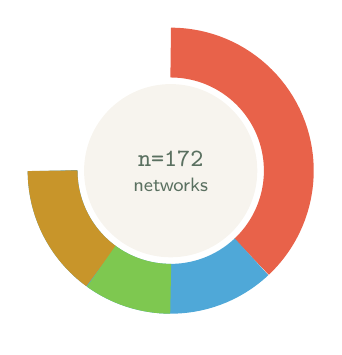
\begin{tikzpicture}
      \def\R{1.5}
      \def\W{0.5}
      % Connector 38% → 136.8°
      \draw[coral, line width=18pt]
        (90:\R) arc (90:-46.8:\R);
      % Specialist 37% → 133.2°
      \draw[sky, line width=18pt]
        (-46.8:\R) arc (-46.8:-180:\R);
      % Keystone 15% → 54°
      \draw[gold, line width=18pt]
        (180:\R) arc (180:234:\R);
      % Generalist 10% → 36°
      \draw[lime, line width=18pt]
        (234:\R) arc (234:270:\R);
      % Inner white fill
      \fill[panel] (0,0) circle (1.1);
      \node[font=\monoFont\fontsize{9}{9}\selectfont\color{muted}] at (0,0.15) {n=172};
      \node[font=\sffamily\fontsize{7}{7}\selectfont\color{muted}] at (0,-0.18) {networks};
    \end{tikzpicture}
    \end{minipage}%
    \begin{minipage}[c]{9in}
      \fontsize{11}{20}\selectfont
      \foreach \col/\lbl/\pct in {
        coral/{Connector}/38,
        sky/{Specialist}/37,
        gold/{Keystone}/15,
        lime/{Generalist}/10}{
        \tikz{\fill[\col, rounded corners=1.5pt] (0,0) rectangle (8pt,8pt);}\enspace
        \lbl\enspace\textbf{\monoFont\color{\col}\pct\%}\\
      }
    \end{minipage}

    \vspace{6pt}
    \begin{minipage}[t]{6.8in}
      \begin{tcolorbox}[
        enhanced, sharp corners, frame hidden,
        colback=panel2, left=6pt, right=6pt, top=5pt, bottom=5pt,
        width=\linewidth]
        {\monoFont\bfseries\fontsize{20}{20}\selectfont\color{headplum} 0.960}\\
        {\fontsize{9}{11}\selectfont\color{muted} Mean GNN AUC\\(171/172 $\geq$ 0.85)}
      \end{tcolorbox}
    \end{minipage}\hspace{0.3in}%
    \begin{minipage}[t]{6.8in}
      \begin{tcolorbox}[
        enhanced, sharp corners, frame hidden,
        colback=panel2, left=6pt, right=6pt, top=5pt, bottom=5pt,
        width=\linewidth]
        {\monoFont\bfseries\fontsize{20}{20}\selectfont\color{teal} 0.384}\\
        {\fontsize{9}{11}\selectfont\color{muted} Mean Silhouette\\score (k=4)}
      \end{tcolorbox}
    \end{minipage}

    \vspace{6pt}
    \begin{tcolorbox}[calloutsky]
      \textbf{Connectance–Generalism:} r = 0.48, p $<$ 0.001.
      Keystone prevalence is connectance-independent (r = 0.07, p = 0.345).
    \end{tcolorbox}
  \end{tcolorbox}
\end{minipage}%
%
\hspace*{0.48in}% gap between col1 and col2
%
% ──────────────── COLUMN 2 ────────────────
\begin{minipage}[t]{\ColW}
  \hspace*{0.0in}

  % ╔══════════════════════════════════╗
  % ║  CARD 4 · Cascading Co-extinction║
  % ╚══════════════════════════════════╝
  \begin{tcolorbox}[
    enhanced, sharp corners, frame hidden,
    colback=panel, left=8pt, right=8pt, top=0pt, bottom=8pt,
    width=15.0in, drop shadow={opacity=0.20},
    before={\vspace{2pt}}, after={\vspace{8pt}}]
    \begin{tcolorbox}[enhanced, sharp corners, frame hidden,
      colback=headcoral, left=8pt, right=8pt, top=4pt, bottom=4pt, width=\linewidth]
      
\begin{tikzpicture}[baseline=(n.base)]
        \node[circle, fill=coral!80, inner sep=0pt, minimum size=14pt,
              font=\monoFont\fontsize{8}{8}\selectfont\bfseries\color{forest}](n){4};
      \end{tikzpicture}\enspace
      {\ebgaramondFont\bfseries\fontsize{14}{16}\selectfont\color{ivory}%
       Cascading Co-extinction}
    \end{tcolorbox}

    \vspace{5pt}
    {\color{bodytext} Pollinators removed sequentially; plants co-extinct when all
     links lost. 50 repeats for random removal average.}

    \vspace{6pt}
    \begin{center}
    \begin{tikzpicture}
      \begin{axis}[
        width=14in, height=7in,
        xmin=0, xmax=1, ymin=0, ymax=1,
        xlabel={\fontsize{9}{9}\selectfont\itshape\color{muted}
                Fraction of pollinators removed},
        ylabel={\fontsize{9}{9}\selectfont\itshape\color{muted}
                Plants surviving},
        xtick={0,0.5,1},
        xticklabels={0, 0.5, 1.0},
        ytick={0,0.25,0.5,0.75,1},
        yticklabels={0, .25, .50, .75, 1.0},
        tick style={draw=none},
        ticklabel style={font=\fontsize{8}{8}\selectfont\color{muted}},
        axis line style={draw=gray!50, line width=0.6pt},
        grid=none,
        clip=false,
        fill between/on layer={axis background},
        axis background/.style={fill=coralbg!60},
      ]
        % 50% threshold
        \addplot[gold, dashed, line width=0.8pt]
          coordinates {(0,0.5)(1,0.5)};
        \node[font=\fontsize{8}{8}\selectfont\color{gold}, anchor=west]
          at (axis cs:1.01,0.5) {50\%};
        % Targeted (red)
        \addplot[coral, line width=2pt, smooth]
          coordinates {
            (0,1.00)(0.08,0.88)(0.16,0.78)(0.24,0.66)(0.32,0.57)
            (0.42,0.46)(0.52,0.38)(0.60,0.32)(0.70,0.26)(0.84,0.22)(1.00,0.18)};
        % Random (blue)
        \addplot[sky, line width=2pt, smooth]
          coordinates {
            (0,1.00)(0.08,0.98)(0.16,0.94)(0.28,0.86)(0.40,0.72)
            (0.52,0.58)(0.62,0.46)(0.72,0.36)(0.82,0.28)(0.92,0.22)(1.00,0.18)};
        % Green fill between
        \addplot[lime!25, fill opacity=0.4]
          fill between[of=rand,of=targ];
        % Half-life markers
        \addplot[coral, dashed, line width=0.7pt]
          coordinates{(0.20,0)(0.20,0.5)};
        \addplot[sky, dashed, line width=0.7pt]
          coordinates{(0.64,0)(0.64,0.5)};
        \node[font=\monoFont\fontsize{8}{8}\selectfont\color{coral}, anchor=north]
          at (axis cs:0.20,0) {\textasciitilde20\%};
        \node[font=\monoFont\fontsize{8}{8}\selectfont\color{sky}, anchor=north]
          at (axis cs:0.64,0) {\textasciitilde65\%};
        % Legend
        \addlegendentry{\fontsize{8.5}{8.5}\selectfont Targeted}
        \addlegendentry{\fontsize{8.5}{8.5}\selectfont Random}
        \pgfplotsset{legend style={
          at={(0.98,0.98)}, anchor=north east,
          fill=white, fill opacity=0.85,
          draw=none, font=\fontsize{8.5}{8.5}\selectfont}}
      \end{axis}
    \end{tikzpicture}
    \end{center}

    \vspace{4pt}
    \begin{tcolorbox}[calloutcoral]
      \textbf{2.5--4$\times$ difference} in network half-life. North America
      (Q=0.270) collapses earliest — targeted removal generates 80--300 isolated
      components.
    \end{tcolorbox}
  \end{tcolorbox}

  % ╔══════════════════════════════════╗
  % ║  CARD 5 · Climate Stress         ║
  % ╚══════════════════════════════════╝
  \begin{tcolorbox}[
    enhanced, sharp corners, frame hidden,
    colback=panel, left=8pt, right=8pt, top=0pt, bottom=8pt,
    width=15.0in, drop shadow={opacity=0.20},
    before={\vspace{2pt}}, after={\vspace{8pt}}]
    \begin{tcolorbox}[enhanced, sharp corners, frame hidden,
      colback=headsky, left=8pt, right=8pt, top=4pt, bottom=4pt, width=\linewidth]
      
\begin{tikzpicture}[baseline=(n.base)]
        \node[circle, fill=sky, inner sep=0pt, minimum size=14pt,
              font=\monoFont\fontsize{8}{8}\selectfont\bfseries\color{forest}](n){5};
      \end{tikzpicture}\enspace
      {\ebgaramondFont\bfseries\fontsize{14}{16}\selectfont\color{ivory}%
       Climate Stress Simulation}
    \end{tcolorbox}

    \vspace{5pt}
    {\color{bodytext} Climate stress modelled as gradual reduction in interaction
     strength (s: 0$\to$1). All networks collapse rapidly beyond s $\approx$ 0.75--0.85.}

    \vspace{6pt}
    \begin{center}
    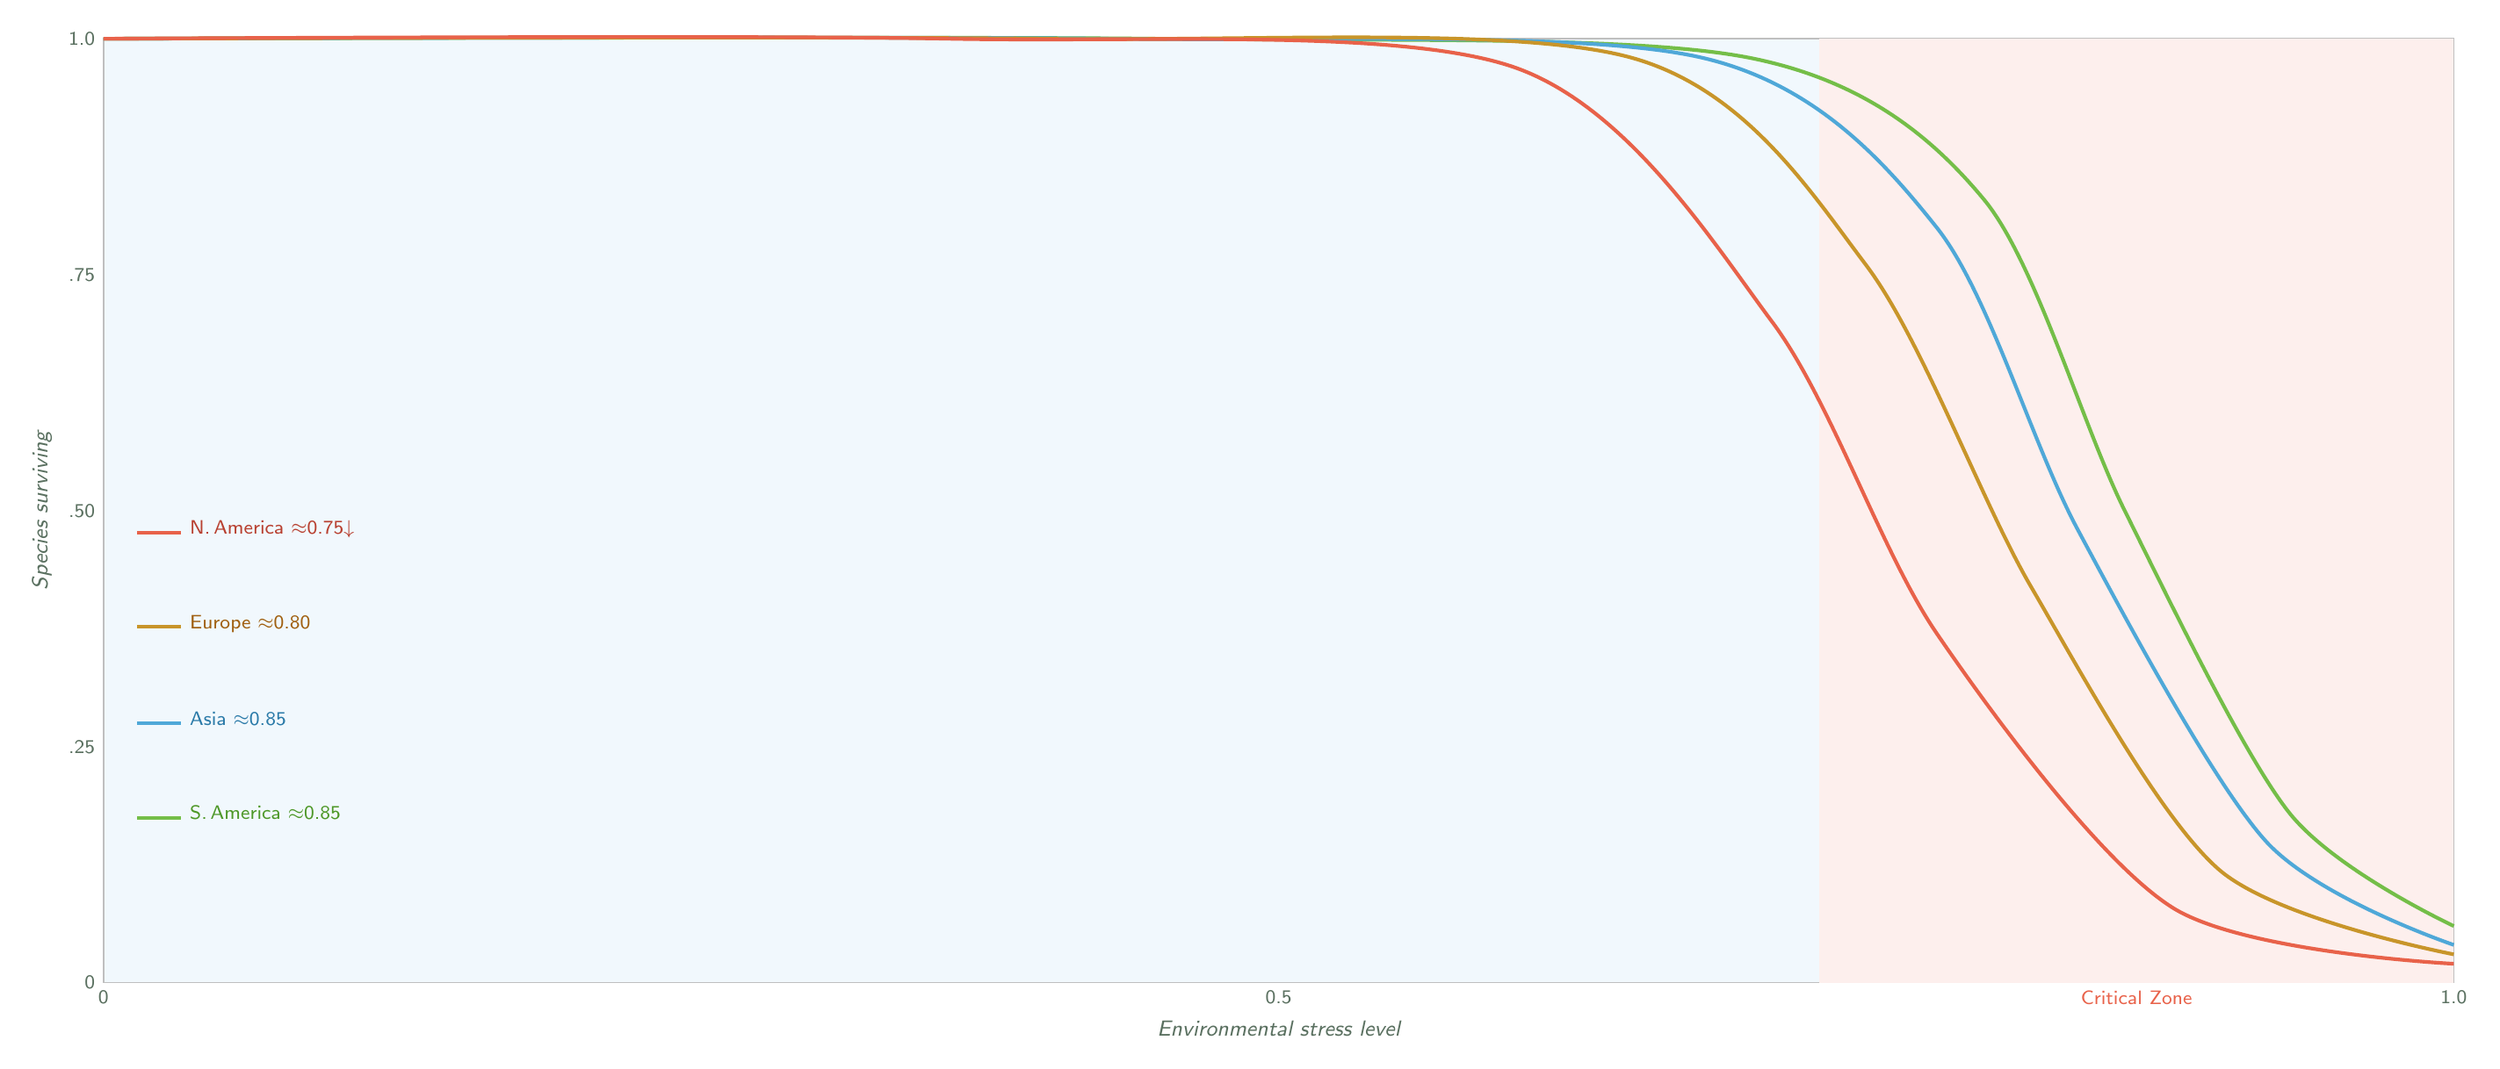
\begin{tikzpicture}
      \begin{axis}[
        width=14in, height=6in,
        xmin=0, xmax=1, ymin=0, ymax=1,
        xlabel={\fontsize{9}{9}\selectfont\itshape\color{muted}
                Environmental stress level},
        ylabel={\fontsize{9}{9}\selectfont\itshape\color{muted}
                Species surviving},
        xtick={0,0.5,1}, ytick={0,0.25,0.5,0.75,1},
        xticklabels={0,0.5,1.0}, yticklabels={0,.25,.50,.75,1.0},
        tick style={draw=none},
        ticklabel style={font=\fontsize{8}{8}\selectfont\color{muted}},
        axis line style={draw=gray!50, line width=0.6pt},
        axis background/.style={fill=skybg!60},
        clip=false,
      ]
        % Critical zone shading
        \fill[coral!10] (axis cs:0.73,0) rectangle (axis cs:1,1);
        \node[font=\fontsize{8}{8}\selectfont\color{coral}, anchor=north]
          at (axis cs:0.865,0) {Critical Zone};
        % S. America ~0.85
        \addplot[lime!80!darkgreen, line width=1.5pt, smooth]
          coordinates{(0,1)(0.45,1)(0.70,0.98)(0.80,0.83)(0.86,0.50)(0.93,0.18)(1,0.06)};
        % Asia ~0.85
        \addplot[sky, line width=1.5pt, smooth]
          coordinates{(0,1)(0.43,1)(0.68,0.98)(0.78,0.80)(0.84,0.48)(0.92,0.15)(1,0.04)};
        % Europe ~0.80
        \addplot[gold, line width=1.5pt, smooth]
          coordinates{(0,1)(0.40,1)(0.65,0.98)(0.75,0.76)(0.82,0.42)(0.90,0.12)(1,0.03)};
        % N. America ~0.75
        \addplot[coral, line width=1.5pt, smooth]
          coordinates{(0,1)(0.36,1)(0.60,0.97)(0.71,0.70)(0.78,0.37)(0.88,0.08)(1,0.02)};
        % Legend lines
        \node[font=\fontsize{8}{8}\selectfont, anchor=west] at (axis cs:0.01,0.18){
          \tikz{\draw[lime!80!darkgreen,line width=1.5pt](0,0)--(18pt,0);}
          \color{darkgreen} S.\,America $\approx$0.85};
        \node[font=\fontsize{8}{8}\selectfont, anchor=west] at (axis cs:0.01,0.28){
          \tikz{\draw[sky,line width=1.5pt](0,0)--(18pt,0);}
          \color{headsky} Asia $\approx$0.85};
        \node[font=\fontsize{8}{8}\selectfont, anchor=west] at (axis cs:0.01,0.38){
          \tikz{\draw[gold,line width=1.5pt](0,0)--(18pt,0);}
          \color{headamber} Europe $\approx$0.80};
        \node[font=\fontsize{8}{8}\selectfont, anchor=west] at (axis cs:0.01,0.48){
          \tikz{\draw[coral,line width=1.5pt](0,0)--(18pt,0);}
          \color{headcoral} N.\,America $\approx$0.75$\downarrow$};
      \end{axis}
    \end{tikzpicture}
    \end{center}

    \vspace{4pt}
    \begin{tcolorbox}[calloutsky]
      \textbf{Pollinators decline before plants} across all networks ---
      monitoring pollinator abundance provides earlier ecosystem stress warning
      than monitoring plant abundance.
    \end{tcolorbox}
  \end{tcolorbox}

  % ╔══════════════════════════════════════╗
  % ║  CARD 6 · Early Warning Signal Det. ║
  % ╚══════════════════════════════════════╝
  \begin{tcolorbox}[
    enhanced, sharp corners, frame hidden,
    colback=panel, left=8pt, right=8pt, top=0pt, bottom=8pt,
    width=15.0in, drop shadow={opacity=0.20},
    before={\vspace{2pt}}, after={\vspace{8pt}}]
    \begin{tcolorbox}[enhanced, sharp corners, frame hidden,
      colback=headamber, left=8pt, right=8pt, top=4pt, bottom=4pt, width=\linewidth]
      
\begin{tikzpicture}[baseline=(n.base)]
        \node[circle, fill=amberlight, inner sep=0pt, minimum size=14pt,
              font=\monoFont\fontsize{8}{8}\selectfont\bfseries\color{forest}](n){6};
      \end{tikzpicture}\enspace
      {\ebgaramondFont\bfseries\fontsize{14}{16}\selectfont\color{ivory}%
       Early Warning Signal Detection}
    \end{tcolorbox}

    \vspace{5pt}
    {\color{bodytext}\textbf{Critical Slowing Down (CSD):} rising variance and
     lag-1 autocorrelation precede collapse bifurcation. CSD autocorrelation
     threshold = 0.9.}

    \vspace{6pt}
    % Dual panel: Variance + Autocorrelation
    \begin{minipage}[t]{6.8in}
      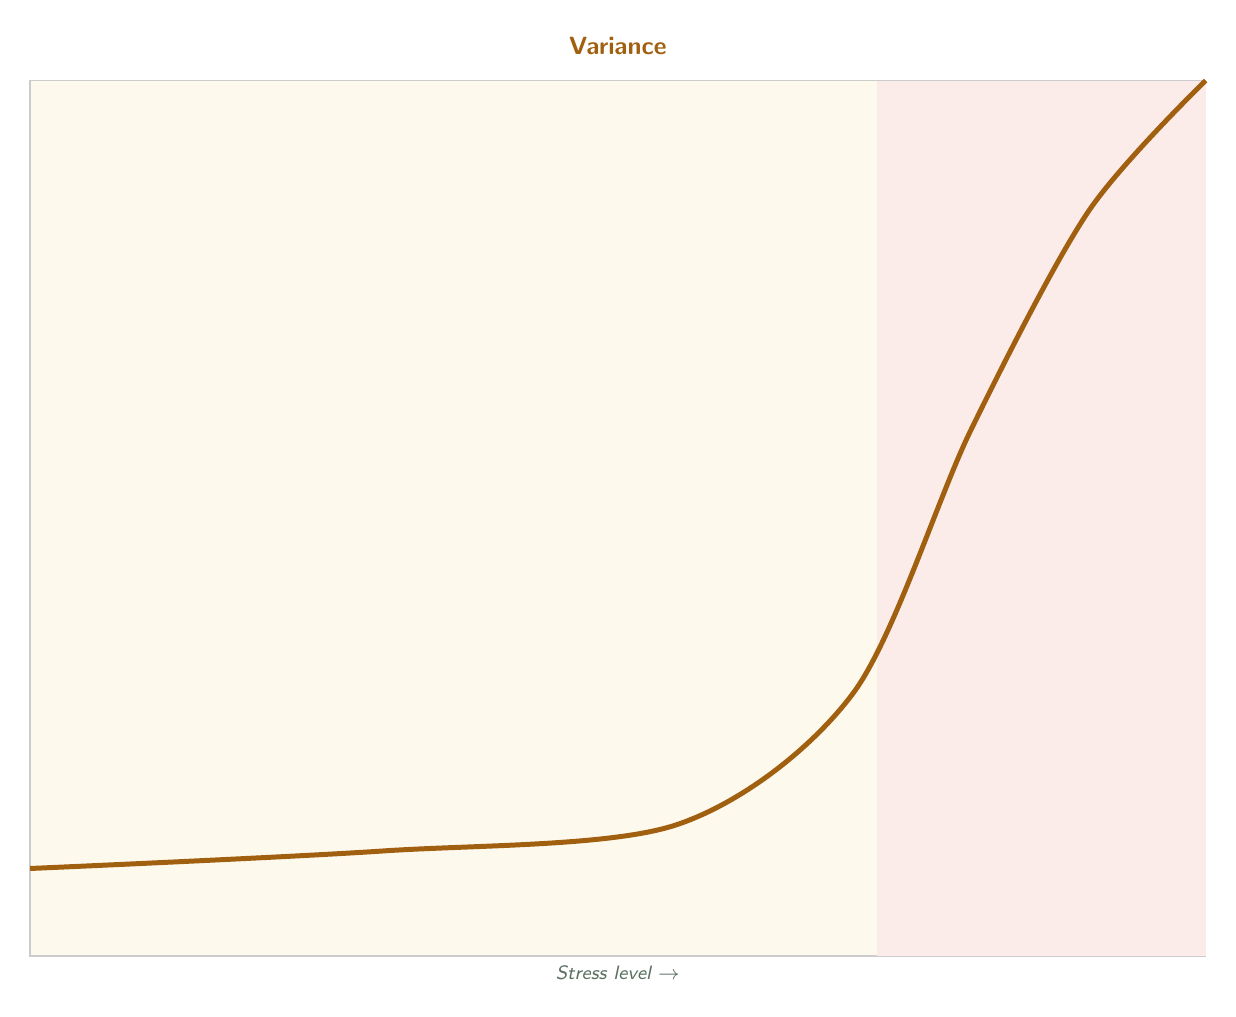
\begin{tikzpicture}
        \begin{axis}[
          width=6.5in, height=5in,
          xmin=0, xmax=1, ymin=0, ymax=1,
          xtick=\empty, ytick=\empty,
          title={\fontsize{9}{9}\selectfont\bfseries\color{headamber} Variance},
          title style={at={(0.5,1.0)}, anchor=south},
          axis background/.style={fill=amberbg!80},
          axis line style={draw=gray!40, line width=0.6pt},
          clip=false,
        ]
          \fill[coral!12] (axis cs:0.72,0) rectangle (axis cs:1,1);
          \addplot[headamber, line width=1.8pt, smooth]
            coordinates{(0,0.10)(0.3,0.12)(0.55,0.15)(0.70,0.30)
                         (0.80,0.60)(0.90,0.85)(1,1)};
          \node[font=\fontsize{7.5}{7.5}\selectfont\itshape\color{muted},
                anchor=north] at (axis cs:0.5,0) {Stress level $\to$};
        \end{axis}
      \end{tikzpicture}
    \end{minipage}\hfill
    \begin{minipage}[t]{6.8in}
      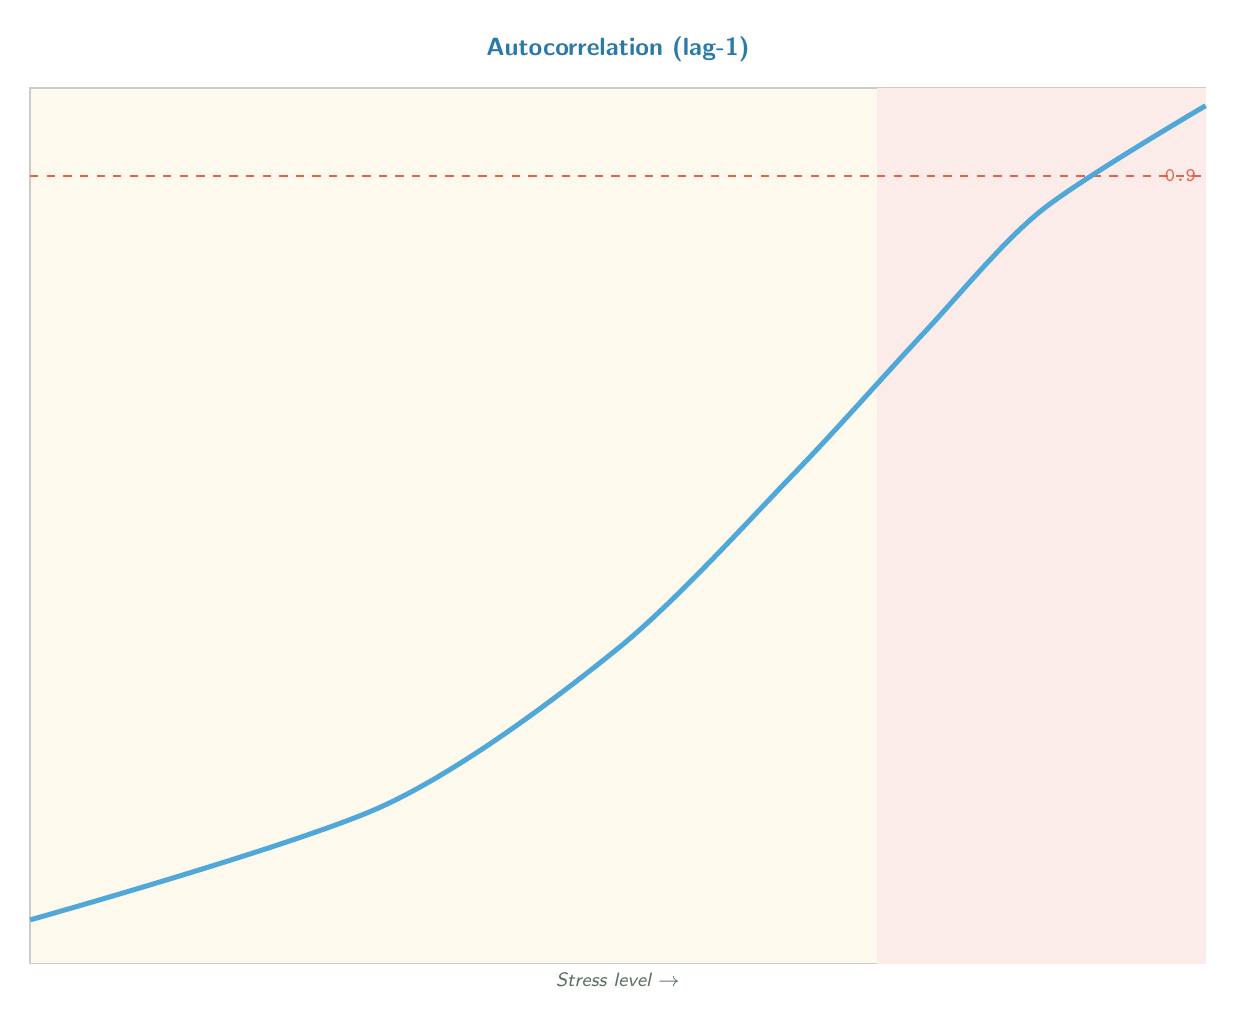
\begin{tikzpicture}
        \begin{axis}[
          width=6.5in, height=5in,
          xmin=0, xmax=1, ymin=0, ymax=1,
          xtick=\empty, ytick=\empty,
          title={\fontsize{9}{9}\selectfont\bfseries\color{headsky}
                 Autocorrelation (lag-1)},
          title style={at={(0.5,1.0)}, anchor=south},
          axis background/.style={fill=amberbg!80},
          axis line style={draw=gray!40, line width=0.6pt},
          clip=false,
        ]
          \fill[coral!12] (axis cs:0.72,0) rectangle (axis cs:1,1);
          \addplot[coral, dashed, line width=0.8pt]
            coordinates{(0,0.9)(1,0.9)};
          \node[font=\monoFont\fontsize{7}{7}\selectfont\color{coral},
                anchor=east] at (axis cs:1,0.9) {0.9};
          \addplot[sky, line width=1.8pt, smooth]
            coordinates{(0,0.05)(0.3,0.18)(0.50,0.36)(0.65,0.56)
                         (0.76,0.72)(0.86,0.86)(1,0.98)};
          \node[font=\fontsize{7.5}{7.5}\selectfont\itshape\color{muted},
                anchor=north] at (axis cs:0.5,0) {Stress level $\to$};
        \end{axis}
      \end{tikzpicture}
    \end{minipage}

    \vspace{5pt}
    \begin{pbullet}
      \item Variance rises at stress \histat{$\approx$ 0.70--0.75}, before
            critical zone at $\sim$0.79
      \item Warning window: \histat{10--30 years} before catastrophic transition
      \item \lostat{Oceania} shows earliest warning — limited island redundancy
    \end{pbullet}
  \end{tcolorbox}

\end{minipage}%
%
\hspace*{0.48in}% gap between col2 and col3
%
% ──────────────── COLUMN 3 ────────────────
\begin{minipage}[t]{14.56in}
  \hspace*{0.0in}

  % ╔══════════════════════════════════════╗
  % ║  CARD 7 · Adaptive Rewiring          ║
  % ╚══════════════════════════════════════╝
  \begin{tcolorbox}[
    enhanced, sharp corners, frame hidden,
    colback=panel, left=8pt, right=8pt, top=0pt, bottom=8pt,
    width=14.0in, drop shadow={opacity=0.20},
    before={\vspace{2pt}}, after={\vspace{8pt}}]
    \begin{tcolorbox}[enhanced, sharp corners, frame hidden,
      colback=headlime, left=8pt, right=8pt, top=4pt, bottom=4pt, width=\linewidth]
      
\begin{tikzpicture}[baseline=(n.base)]
        \node[circle, fill=lime, inner sep=0pt, minimum size=14pt,
              font=\monoFont\fontsize{8}{8}\selectfont\bfseries\color{forest}](n){7};
      \end{tikzpicture}\enspace
      {\ebgaramondFont\bfseries\fontsize{14}{16}\selectfont\color{ivory}%
       Adaptive Rewiring (p = 0.6)}
    \end{tcolorbox}

    \vspace{5pt}
    {\color{bodytext} Surviving plants seek alternative pollinators proportional
     to degree when a partner is lost. Resilience gain = area between rewiring
     and no-rewiring curves.}

    \vspace{6pt}
    \begin{center}
    \begin{tikzpicture}
      \begin{axis}[
        width=13in, height=5.5in,
        xmin=0, xmax=1, ymin=0, ymax=1,
        xlabel={\fontsize{9}{9}\selectfont\itshape\color{muted}
                Fraction of pollinators removed $\to$},
        ylabel={\fontsize{9}{9}\selectfont\itshape\color{muted}
                Plants surviving},
        xtick=\empty, ytick=\empty,
        axis background/.style={fill=limebg!80},
        axis line style={draw=gray!40, line width=0.6pt},
        clip=false,
      ]
        % resilience-gain fill
        \addplot[lime!30, fill opacity=0.45]
          fill between[of=rewire,of=norewire];
        % With rewiring
        \addplot[darkgreen, line width=2pt, smooth, name path=rewire]
          coordinates{(0,0.92)(0.15,0.82)(0.30,0.70)(0.48,0.54)
                       (0.65,0.40)(0.82,0.28)(1,0.18)};
        % Without rewiring
        \addplot[coral, dashed, line width=2pt, smooth, name path=norewire]
          coordinates{(0,0.82)(0.15,0.68)(0.30,0.55)(0.48,0.42)
                       (0.65,0.32)(0.82,0.24)(1,0.18)};
        \node[font=\fontsize{8}{8}\selectfont\bfseries\color{darkgreen},
              anchor=west] at (axis cs:0.60,0.44) {With rewiring};
        \node[font=\fontsize{8}{8}\selectfont\color{coral},
              anchor=west] at (axis cs:0.60,0.29) {No rewiring};
        \node[font=\fontsize{8}{8}\selectfont\itshape\color{darkgreen},
              anchor=center] at (axis cs:0.33,0.65) {resilience gain};
      \end{axis}
    \end{tikzpicture}
    \end{center}

    \vspace{4pt}
    \begin{pbullet}
      \item \textbf{Largest gain:} Europe \& Oceania (high nestedness)
      \item \textbf{Smallest:} Asia \& N.\,America (modular, locally saturated)
      \item Benefit positively correlated with nestedness
    \end{pbullet}
    \vspace{4pt}
    \begin{tcolorbox}[calloutteal]
      \textbf{Conservation:} Habitat corridors enabling pollinators to encounter
      novel plants significantly boost resilience beyond species-level protection.
    \end{tcolorbox}
  \end{tcolorbox}

  % ╔══════════════════════════════════════╗
  % ║  CARD 8 · ML Extinction Risk Pred.  ║
  % ╚══════════════════════════════════════╝
  \begin{tcolorbox}[
    enhanced, sharp corners, frame hidden,
    colback=panel, left=8pt, right=8pt, top=0pt, bottom=8pt,
    width=14.0in, drop shadow={opacity=0.20},
    before={\vspace{2pt}}, after={\vspace{8pt}}]
    \begin{tcolorbox}[enhanced, sharp corners, frame hidden,
      colback=headgold, left=8pt, right=8pt, top=4pt, bottom=4pt, width=\linewidth]
      
\begin{tikzpicture}[baseline=(n.base)]
        \node[circle, fill=gold2, inner sep=0pt, minimum size=14pt,
              font=\monoFont\fontsize{8}{8}\selectfont\bfseries\color{forest}](n){8};
      \end{tikzpicture}\enspace
      {\ebgaramondFont\bfseries\fontsize{14}{16}\selectfont\color{ivory}%
       ML Extinction Risk Prediction}
    \end{tcolorbox}

    \vspace{5pt}
    {\color{bodytext}\textbf{Random Forest} classifier (100 trees, 5-fold CV) on
     structural node features. Consistent feature importance across all 6
     continental networks.}

    \vspace{6pt}
    % Horizontal bar chart
    \begin{center}
    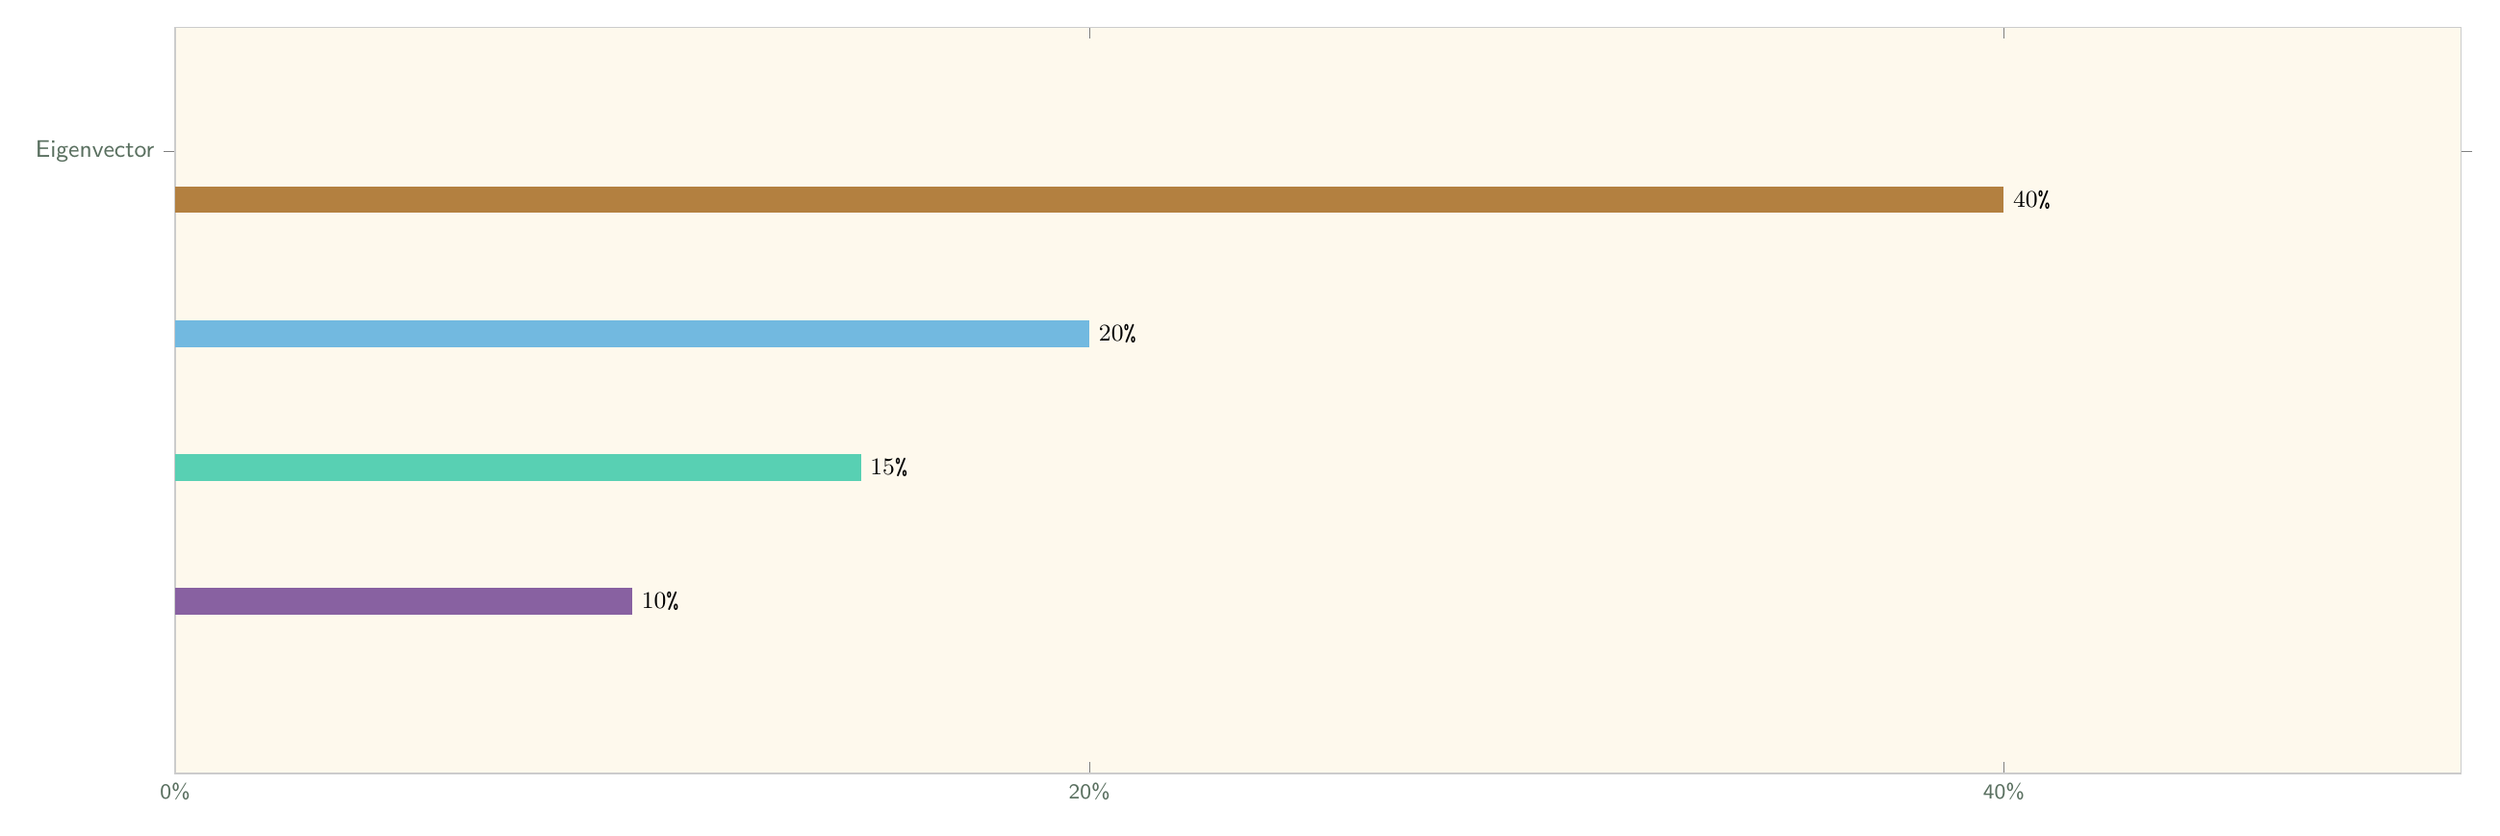
\begin{tikzpicture}
      \begin{axis}[
        xbar,
        width=12.5in, height=4.5in,
        xmin=0, xmax=50,
        symbolic y coords={Module conn., Betweenness, Degree, Eigenvector},
        ytick=data,
        yticklabel style={font=\fontsize{9}{9}\selectfont\color{muted}, anchor=east},
        xtick={0,20,40},
        xticklabels={0\%,20\%,40\%},
        ticklabel style={font=\fontsize{8}{8}\selectfont\color{muted}},
        axis background/.style={fill=amberbg!80},
        axis line style={draw=gray!40, line width=0.6pt},
        enlarge y limits=0.25,
        nodes near coords={\pgfmathprintnumber\pgfplotspointmeta\%},
        nodes near coords style={
          font=\monoFont\bfseries\fontsize{9}{9}\selectfont,
          anchor=west},
        clip=false,
      ]
        \addplot[fill=headamber!80, draw=none, point meta=explicit]
          coordinates {(40,Eigenvector)[40]};
        \addplot[fill=sky!80, draw=none, point meta=explicit]
          coordinates {(20,Degree)[20]};
        \addplot[fill=teal!80, draw=none, point meta=explicit]
          coordinates {(15,Betweenness)[15]};
        \addplot[fill=headplum!80, draw=none, point meta=explicit]
          coordinates {(10,{Module conn.})[10]};
      \end{axis}
    \end{tikzpicture}
    \end{center}

    \vspace{4pt}
    \begin{tcolorbox}[calloutgold]
      \textbf{Eigenvector dominates ($\approx$40\%).} Conserving pollinators
      by interaction frequency alone misses systemically critical species at
      strategic positions.
    \end{tcolorbox}
  \end{tcolorbox}

  % ╔══════════════════════════════════════╗
  % ║  CARD 9 · Species Transplantation   ║
  % ╚══════════════════════════════════════╝
  \begin{tcolorbox}[
    enhanced, sharp corners, frame hidden,
    colback=panel, left=8pt, right=8pt, top=0pt, bottom=8pt,
    width=14.0in, drop shadow={opacity=0.20},
    before={\vspace{2pt}}, after={\vspace{8pt}}]
    \begin{tcolorbox}[enhanced, sharp corners, frame hidden,
      colback=headcoral, left=8pt, right=8pt, top=4pt, bottom=4pt, width=\linewidth]
      
\begin{tikzpicture}[baseline=(n.base)]
        \node[circle, fill=coral!80, inner sep=0pt, minimum size=14pt,
              font=\monoFont\fontsize{8}{8}\selectfont\bfseries\color{forest}](n){9};
      \end{tikzpicture}\enspace
      {\ebgaramondFont\bfseries\fontsize{14}{16}\selectfont\color{ivory}%
       Species Transplantation}
    \end{tcolorbox}

    \vspace{5pt}
    {\color{bodytext} Introduced \emph{``Unidentified sp16 M\_PL\_050''} into
     M\_PL\_050 target community (17 plants $\times$ 51 pollinators).}

    \vspace{6pt}
    % Before / After mini network diagrams
    \begin{minipage}[t]{6in}
      \begin{center}
      {\fontsize{9}{9}\selectfont\bfseries\color{muted} BEFORE}\\[4pt]
      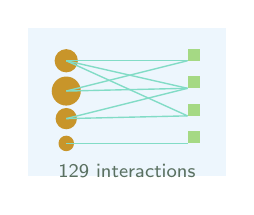
\begin{tikzpicture}[scale=0.7]
        \fill[skybg!80] (-1.5,-2.1) rectangle (2.1,0.6);
        \foreach \y/\r in {0/6pt, -0.55/7.5pt, -1.05/5.5pt, -1.5/4pt}
          \fill[gold] (-0.8,\y) circle (\r);
        \foreach \y in {0, -0.5, -1.0, -1.5}
          \fill[lime!70] (1.4,\y) rectangle ++(0.22, 0.22);
        \foreach \py/\vy in {
          0/0, 0/-0.5, 0/-1.0, -0.55/0, -0.55/-0.5,
          -1.05/-0.5, -1.05/-1.0, -1.5/-1.5}
          \draw[teal!60, line width=0.5pt] (-0.8,\py) -- (1.4,\vy);
        \node[font=\fontsize{7}{7}\selectfont\color{muted}] at (0.3,-2.0) {129 interactions};
      \end{tikzpicture}
      \end{center}
    \end{minipage}\hfill
    \begin{minipage}[t]{6in}
      \begin{center}
      {\fontsize{9}{9}\selectfont\bfseries\color{muted} AFTER}\\[4pt]
      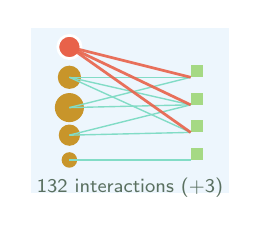
\begin{tikzpicture}[scale=0.7]
        \fill[skybg!80] (-1.5,-2.1) rectangle (2.1,0.9);
        \foreach \y/\r in {0/6pt, -0.55/7.5pt, -1.05/5.5pt, -1.5/4pt}
          \fill[gold] (-0.8,\y) circle (\r);
        % Transplant node (red)
        \fill[coral] (-0.8,0.55) circle (6pt);
        \draw[white, line width=1pt] (-0.8,0.55) circle (6pt);
        \foreach \y in {0, -0.5, -1.0, -1.5}
          \fill[lime!70] (1.4,\y) rectangle ++(0.22, 0.22);
        \foreach \py/\vy in {
          0/0, 0/-0.5, 0/-1.0, -0.55/0, -0.55/-0.5,
          -1.05/-0.5, -1.05/-1.0, -1.5/-1.5}
          \draw[teal!60, line width=0.5pt] (-0.8,\py) -- (1.4,\vy);
        % New links (red)
        \foreach \vy in {0, -0.5, -1.0}
          \draw[coral, line width=1pt, opacity=0.9] (-0.8,0.55) -- (1.4,\vy);
        \node[font=\fontsize{7}{7}\selectfont\color{muted}] at (0.3,-2.0) {132 interactions (+3)};
      \end{tikzpicture}
      \end{center}
    \end{minipage}

    \vspace{6pt}
    \renewcommand{\arraystretch}{1.15}
    \fontsize{10}{13}\selectfont
    \begin{tabularx}{\linewidth}{X r r >{\bfseries}r}
      \rowcolor{darkgrn}%
      \textcolor{gold2}{\small Metric} &
      \textcolor{gold2}{\small Before} &
      \textcolor{gold2}{\small After} &
      \textcolor{gold2}{\small $\Delta$} \\
      Interactions & 129    & 132    & \textcolor{teal}{+3} \\
      \rowcolor{panel2}
      NODF         & 38.94  & 38.06  & \textcolor{coral}{$-$0.88} \\
      Modularity Q & 0.4627 & 0.4502 & \textcolor{coral}{$-$0.013} \\
      \rowcolor{panel2}
      LCC Size     & 68     & 69     & \textcolor{teal}{+1} \\
    \end{tabularx}

    \vspace{6pt}
    \begin{tcolorbox}[calloutcoral]
      \textbf{Key constraint:} transplanted species must target bridge plants
      (high betweenness) — not over-connected nodes — to improve resilience.
    \end{tcolorbox}
  \end{tcolorbox}

\end{minipage}%

} % end font group

% ════════════════════════════════════════════════════════
%   FINDINGS STRIP + FOOTER  (TikZ overlay, bottom portion)
% ════════════════════════════════════════════════════════
\begin{tikzpicture}[remember picture, overlay,
    every node/.style={inner sep=0pt, outer sep=0pt}]

  % ── Findings strip background ─────────────────────────
  \fill[white]  ($(BL)+(0,3.60in)$) rectangle ++(48in,3.50in);
  \fill[panel2!50] ($(BL)+(0,4.10in)$) rectangle ++(48in,3.0in);
  \draw[gold, line width=2pt] ($(BL)+(0,7.10in)$) -- ++(48in,0);
  \draw[gold!40, line width=0.8pt] ($(BL)+(0,3.60in)$) -- ++(48in,0);

  % Label
  \node[anchor=center,
        font=\ebgaramondFont\bfseries\fontsize{12}{12}\selectfont\color{gold2},
        opacity=0.85]
    at ($(BL)+(24in,6.90in)$)
    {{\fontsize{8}{8}\selectfont\color{gold}$\blacklozenge$}\quad
     KEY FINDINGS \& CONCLUSIONS\quad
     {\fontsize{8}{8}\selectfont\color{gold}$\blacklozenge$}};

  % Findings dividers
  \draw[gold!30, line width=0.6pt]
    ($(BL)+(16in,3.60in)$) -- ++(0,3.50in);
  \draw[gold!30, line width=0.6pt]
    ($(BL)+(32in,3.60in)$) -- ++(0,3.50in);

  % Finding 01
  \node[anchor=north west,
        font=\ebgaramondFont\bfseries\fontsize{48}{48}\selectfont\color{gold!25}]
    at ($(BL)+(0.6in,6.65in)$) {01};
  \node[anchor=north west,
        font=\ebgaramondFont\bfseries\fontsize{14}{16}\selectfont\color{gold2},
        text width=14.5in]
    at ($(BL)+(0.6in,6.0in)$) {Continental Architecture Diversity};
  \node[anchor=north west,
        font=\sffamily\fontsize{10.5}{14.5}\selectfont\color{bodytext},
        text width=14.5in]
    at ($(BL)+(0.6in,5.62in)$)
    {\textbf{South America} (Q=0.773) most stress-resistant.
     \textbf{North America} (Q=0.270) most vulnerable — 2.5--4$\times$ faster
     collapse under targeted vs. random removal. Africa's high nestedness
     (NODF=18.2) drives synchronous tipping-point collapse.};

  % Finding 02
  \node[anchor=north west,
        font=\ebgaramondFont\bfseries\fontsize{48}{48}\selectfont\color{gold!25}]
    at ($(BL)+(16.6in,6.65in)$) {02};
  \node[anchor=north west,
        font=\ebgaramondFont\bfseries\fontsize{14}{16}\selectfont\color{gold2},
        text width=14.5in]
    at ($(BL)+(16.6in,6.0in)$) {GNN Corpus \& Eigenvector Dominance};
  \node[anchor=north west,
        font=\sffamily\fontsize{10.5}{14.5}\selectfont\color{bodytext},
        text width=14.5in]
    at ($(BL)+(16.6in,5.62in)$)
    {Across 172 networks, \textbf{Connector (38\%)} and \textbf{Specialist (37\%)}
     are co-dominant regimes. \textbf{Eigenvector centrality} consistently
     outperforms raw degree as extinction risk predictor ($\sim$40\% RF importance),
     arguing for eigenvector-based conservation prioritisation.};

  % Finding 03
  \node[anchor=north west,
        font=\ebgaramondFont\bfseries\fontsize{48}{48}\selectfont\color{gold!25}]
    at ($(BL)+(32.6in,6.65in)$) {03};
  \node[anchor=north west,
        font=\ebgaramondFont\bfseries\fontsize{14}{16}\selectfont\color{gold2},
        text width=14.5in]
    at ($(BL)+(32.6in,6.0in)$) {Early Warning \& Rewiring Buffer};
  \node[anchor=north west,
        font=\sffamily\fontsize{10.5}{14.5}\selectfont\color{bodytext},
        text width=14.5in]
    at ($(BL)+(32.6in,5.62in)$)
    {\textbf{CSD signals} detectable \textbf{10--30 years} before catastrophic
     collapse. \textbf{Adaptive rewiring} improves resilience across all networks
     — highest in nested communities. \textbf{Managed transplantation} modestly
     improves resilience when species bridges structural gaps.};

  % ── Footer ───────────────────────────────────────────
  \fill[white] (BL) rectangle ++(48in,3.60in);
  \draw[gold!30, line width=0.6pt] ($(BL)+(0,3.60in)$) -- ++(48in,0);

  % Reference
  \node[anchor=north west,
        font=\sffamily\bfseries\fontsize{8}{8}\selectfont\color{forest!80},
        text depth=0]
    at ($(BL)+(0.5in,3.40in)$) {\MakeUppercase{Reference}};
  \node[anchor=north west,
        font=\sffamily\fontsize{8}{11.5}\selectfont\color{forest!72},
        text width=36in]
    at ($(BL)+(0.5in,3.08in)$)
    {[1]\enspace J.\,Bascompte, P.\,Jordano, C.\,J.\,Melian, and
     J.\,M.\,Olesen, ``The nested assembly of plant-animal mutualistic
     networks,'' \textit{Proc. Natl. Acad. Sci. U.S.A.},
     vol.\,100, no.\,16, pp.\,9383--9387, 2003.};

  \node[anchor=north west,
        font=\sffamily\fontsize{8}{11.5}\selectfont\color{forest!72},
        text width=36in]
    at ($(BL)+(0.5in,2.40in)$)
    {\textbf{Data Source:}\enspace Web of Life (www.web-of-life.es)};

  % Contact / institution
  \node[anchor=north east,
        align=right,
        font=\sffamily\fontsize{9.5}{16}\selectfont\color{forest!72}]
    at ($(BR)+(-0.5in,3.40in)$)
    {{\color{gold2}\textbf{IIT Bhilai · Dept. of CSE}}\\
     Network Science Project\\
     Bhilai, Chhattisgarh · April 2026};

\end{tikzpicture}

\end{frame}
\end{document}